% !TEX root = ../main.tex

\chapter{Konzeption \& Design}
\label{ch:KuD}

Nachdem in den vorherigen Kapiteln die Grundlagen gelegt und die Lücken der bestehenden Systeme analysiert wurden, wird nun der Entwurf der Lösung thematisiert. In diesem Kapitel wird der Entwurf des Frameworks zur automatisierten Architekturvalidierung von Anforderung bis zum detaillierten Design nachvollziehbar dargelegt. Im ersten Abschnitt werden daher die Spezifikationen der funktionalen und nicht-funktionalen Anforderungen präsentiert. Auf dieser Basis wird anschließend der Architekturentwurf vorgestellt, welcher die Einbettung in das übergeordnete System erläutert. Die nachfolgenden Abschnitte fokussieren diesen Entwurf durch die detaillierte Konzeption der Programmierschnittstelle sowie dem Design der grafischen Benutzeroberfläche.


\section{Anforderungsanalyse}
\label{sec:Anforderungsanalyse}

Eine präzise Definition der Anforderungen ist die zwingende Voraussetzung für eine zielgerichtete Entwicklung. Basierend auf der Analyse der bestehenden Systemlücke werden daher die funktionalen und nicht-funktionalen Anforderungen an das zu entwickelnde Framework in Tabelle~\ref{tab:anforderungen} spezifiziert. Diese bilden die verbindliche Grundlage für alle nachfolgenden Design- und Implementierungsentscheidungen.

\begin{table}[ht!]
  \centering
  \footnotesize
  \begin{tabularx}{\textwidth}{l l X}
    \toprule
    \textbf{ID} & \textbf{Anforderung}           & \textbf{Beschreibung}                                                                                                                                                                   \\
    \midrule
    \multicolumn{3}{c}{\textit{Funktional}}                                                                                                                                                                                                \\
    \midrule
    FA-1        & Algorithmen-API                & Bereitstellung einer API, die es Nutzern ermöglicht, Validierungsalgorithmen zu verwalten (hochladen, bearbeiten, löschen) und auszuführen.                                             \\
    \midrule
    FA-2        & Algorithmenverwaltung-GUI      & Bereitstellung einer \gls{gui} zur Verwaltung von Validierungsalgorithmen. Diese muss Funktionen zum Hochladen, Bearbeiten, Löschen sowie zum Starten der Ausführung umfassen.          \\
    \midrule
    FA-3        & Ergebniss-GUI                  & Bereitstellung einer \gls{gui} zur visuellen Darstellung der Ergebnisse von Validierungsläufen. Die \gls{gui} muss verschiedene Ausgabeformate (z. B. textuell, grafisch) unterstützen. \\
    \midrule
    FA-4        & Erster Validierungsalgorithmus & Bereitstellung eines ersten Validierungsalgorithmus, der eine grundlegende Architekturprüfung durchführt.                                                                               \\
    \bottomrule
    \multicolumn{3}{c}{\textit{Nicht-Funktional}}                                                                                                                                                                                          \\
    \midrule
    NFA-1       & Standardisierte API            & Die zu entwickelnde API muss den Prinzipien des \gls{rest}folgen.                                                                                                                       \\
    \midrule
    NFA-2       & Benutzerfreundlichkeit         & Die GUI muss intuitiv bedienbar sein.                                                                                                                                                   \\
    \bottomrule
  \end{tabularx}
  \caption{Anforderungen an das Framework}
  \label{tab:anforderungen}
\end{table}

Im Folgenden wird die Notwendigkeit für jede dieser Anforderungen näher erläutert.

\subsection*{Algorithmen-\gls{api}}

Ein zentrales Element des Frameworks ist die Bereitstellung der \gls{api}, um die Validierungsalgorithmen an das ArchitekturTool binden zu können (FA-1). Diese Funktion ist die Grundvoraussetzung, um das System, wie im Ziel der Arbeit gefordert, erweiterbar zu gestalten. Um die Integration weiterer bzw. Anpassung bestehender Funktionalitäten für Entwickler zu vereinfachen und eine hohe Kompatibilität zu gewährleisten, wird zudem die Einhaltung des \gls{rest}-Standards gefordert (NFA-1). Dieser etablierte Standard fördert eine lose Kopplung zwischen Framework und den angebundenen Algorithmen und ermöglicht eine schnelle Einarbeitung für Entwickler, die nicht vertraut sind mit dem Programm.

\subsection*{Grafische Benutzeroberfläche}

Für die Interaktion mit dem Nutzer ist eine grafische Benutzeroberfläche zur Verwaltung der Algorithmen essenziell (FA-2). Sie muss alle notwendigen Funktionen wie das Hochladen und Ausführen der Validierungsalgorithmen ermöglichen. Um einen reibungslosen Ablauf beim benutzen des Tools zu gewährleisten, muss die Bedienung intuitiv und selbterklärend sein (NFA-2). Die Benutzerfreundlichkeit ist entscheidend für die Ingenieure und Entwickler im Arbteitsalltag. Des Weiteren müssen die Ergebnisse der Architekturvaliderungen visuell aufbereitet und ausgegeben werden (FA-3). Ohne eine Visualisierung der Ergebnisse ist es für den Nutzer schwer ersichtlich, was genau die Validierung ergeben hat. Die Unterstützung verschiedener Visualisierungsarten, wie textueller oder grafischer Ausgaben, ermöglichen es dem Nutzer, die Fehlerursache bzw. den Engpass effizient zu identifizieren.

\subsection*{Erster Validierungsalgorithmus}

Das Anbinden eines ersten Validierungsalgorithmus (FA-4) ist aus mehreren Gründen wichtig. Zum einen lässt sich damit das Framework auf Korrektheit prüfen, sprich es dient als Proof of Concept. Mit einem Validierungsalgorithmus lässt sich zum einen prüfen, ob das Hochladen, Bearbeiten und Ausführen der \gls{api} wie gefordert funktioniert. Zum anderen können  zukünftige Ingenieure und Entwickler den Algorithmus als Referenz nutzen um weitere Algorithmen anzubinden.Schließlich ermöglicht dieser erste Algorithmus die Durchführung von aussagekräftigen Tests und bildet die Grundlage für die Evaluation dieser Arbeit.

\section{Systemarchitektur}

Bei dem bestehenden ArchitekturTool handelt es sich um eine dockerisierte Webanwendung, deren Architektur auf einem React-Frontend, einem Node.js-Backend mit dem Express-Framework und einer PostgreSQL-Datenbank mit Prisma-ORM basiert. Um die geforderte Architekturvalidierung zu realisieren, wird diese Architektur, wie in Abbildung~\ref{fig:blockdiagram} dargestellt, um eine dedizierte Validierungs-\gls{api} sowie um zugehörige Frontend-Module erweitert.


\begin{figure}[h!]
  \centering
  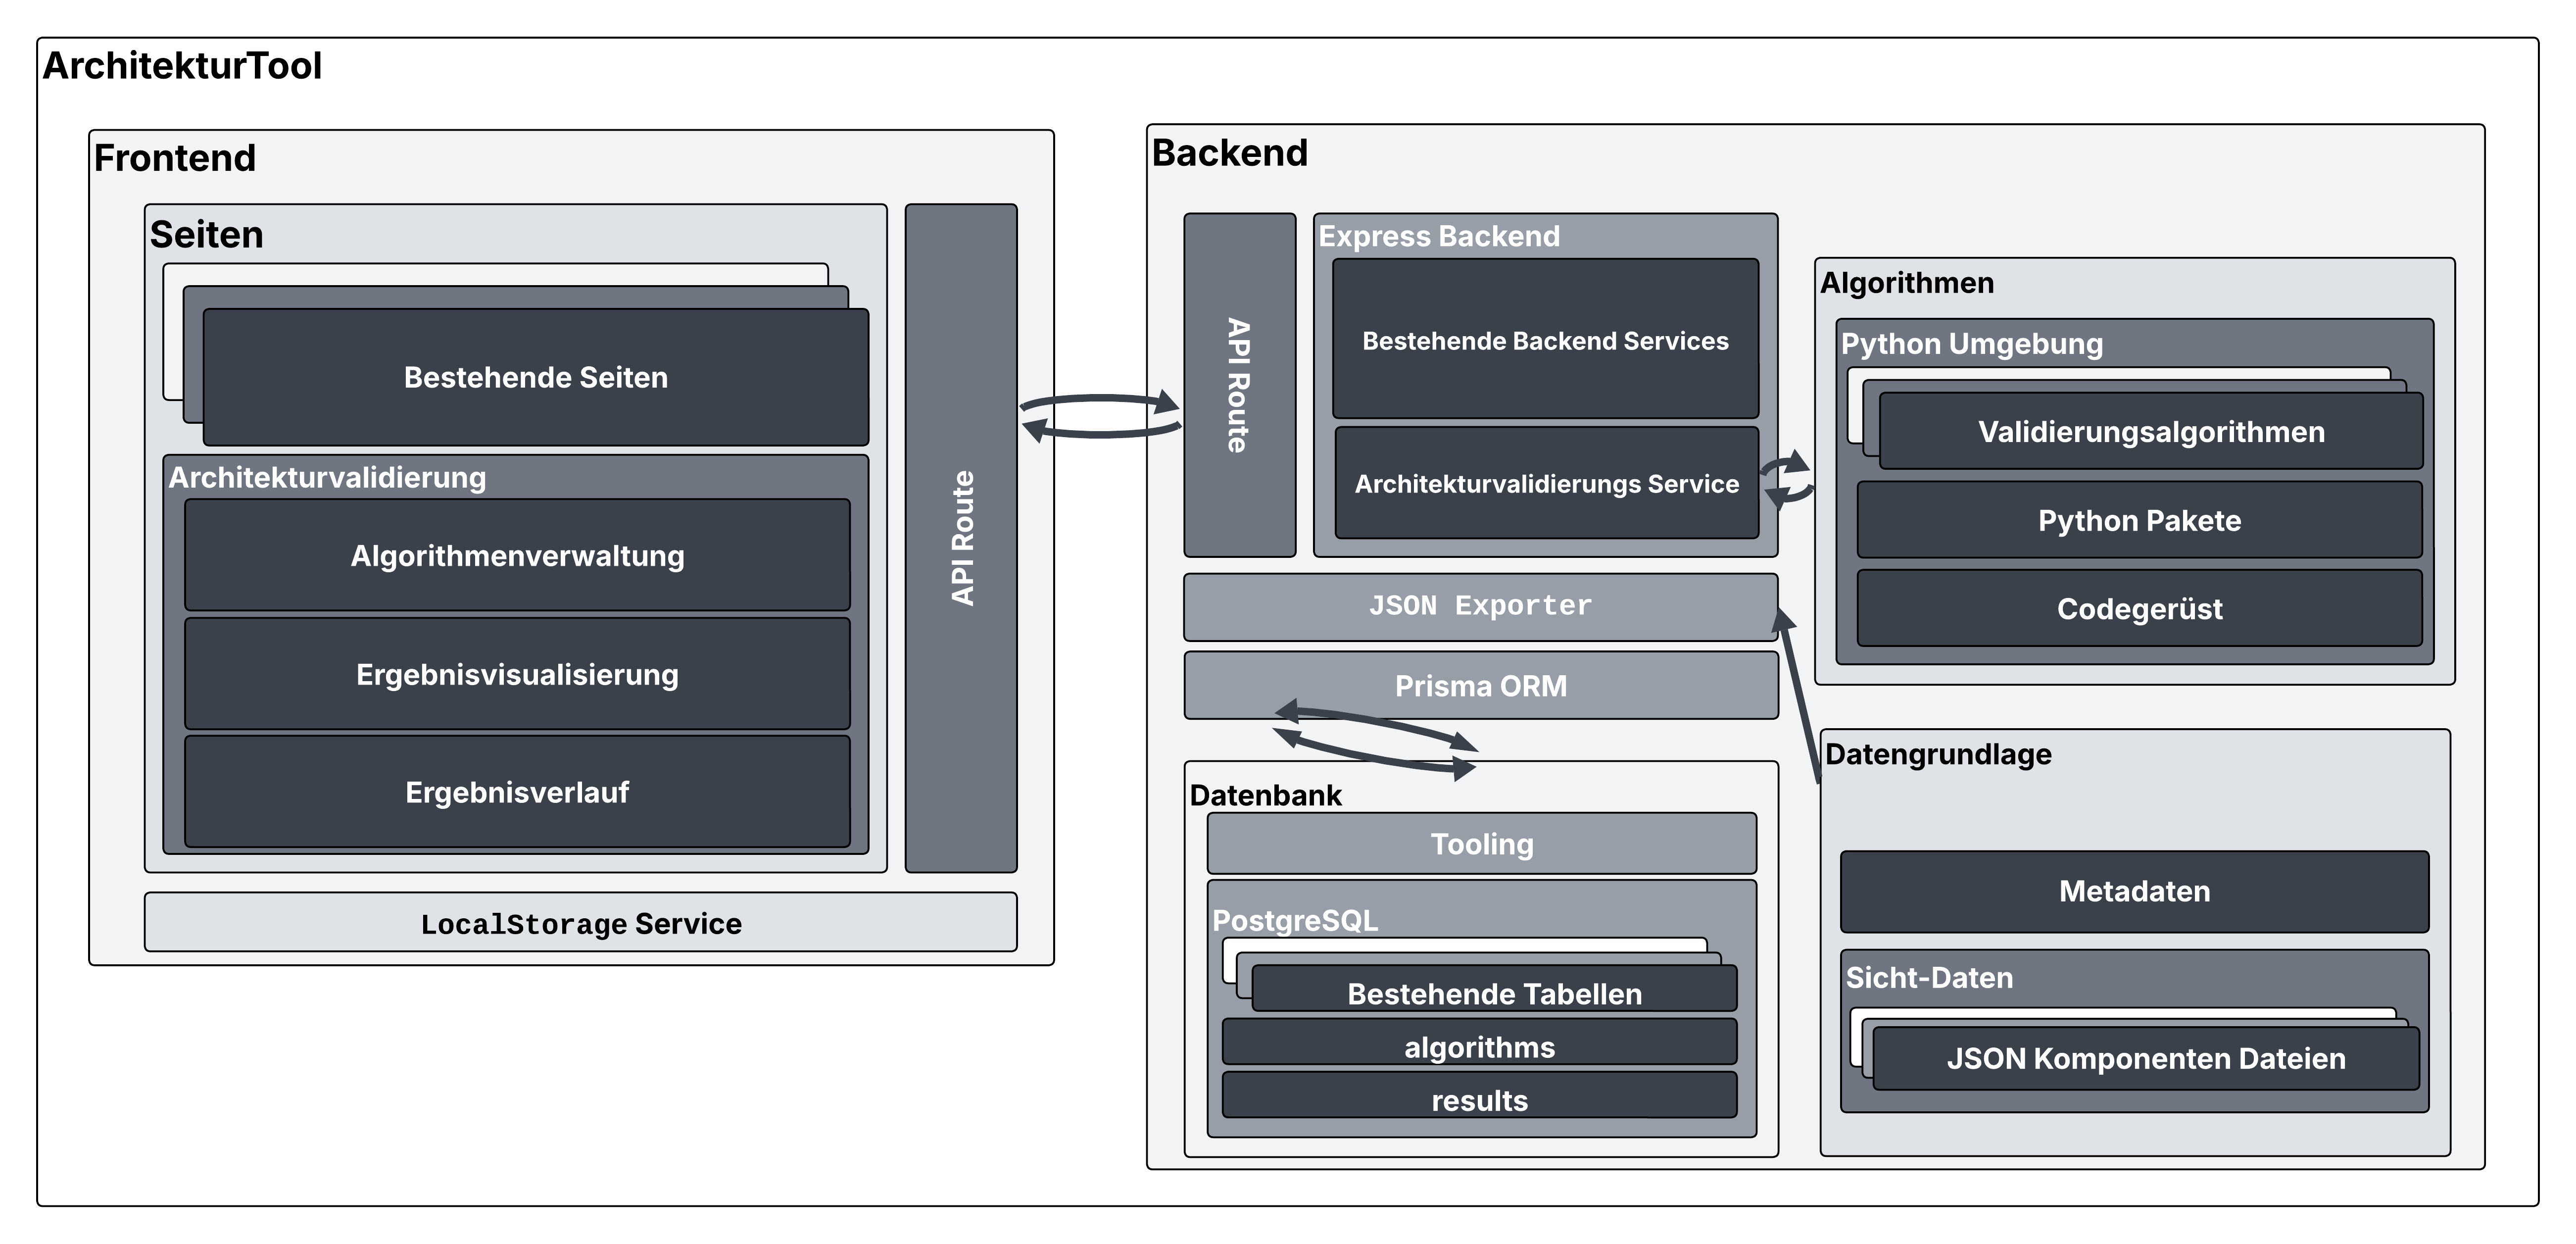
\includegraphics[width=\textwidth]{figures/04Konzeption/Blockdiagram.png}
  \caption{Blockdiagramm des ArchitekturTool's}
  \label{fig:blockdiagram}
\end{figure}


Wie im Blockdiagramm dargestellt, lässt sich die Erweiterung in vier Hauptbereiche unterteilen:

\subsection*{Algorithmenverwaltung (Frontend)}

Diese Komponente bildet die zentrale Verwaltungseinheit für den Nutzer. Es stellt eine Benutzeroberfläche zur Verfügung, um Validierungsalgorithmen zu verwalten (hochladen, bearbeiten, löschen). Darüber hinaus ermöglicht es dem Nutzer, einen hochgeladenen Algorithmus und eine im ArchitekturTool spezifizierte Sicht auszuwählen und einen Validierungslauf zu starten.

\subsection*{Ergebnisvisualisierung (Frontend)}

Diese Komponente ist ausschließlich für die Darstellung der Validierungsergebnisse zuständig. Es bereitet die Ergebnisse eines Validierungslauf auf und stellt sie dem Nutzer, je nach Definierung, in textueller, beispielsweise als Fehlerlist, oder als grafischer Visualisierung, zum Beispiel als Balkendiagramm,  vor.

\subsection*{Validierungsalgorithmus-API (Backend)}



\subsection*{Validierung-Ausführen (Backend)}

\section{Konzeption der Komponenten}



\subsection{Programmierschnittstelle}


\subsection{Grafische Benutzeroberfläche}



\subsection{Validierungsalgorithmus}